\documentclass[compress,xcolor=table]{beamer}

% Packages
\usepackage[french]{babel}
\usepackage[utf8]{inputenc}
\usepackage[T1]{fontenc}
\usepackage{datetime}
\usepackage{fourier}
\usepackage{graphicx}
\usepackage{subcaption}
\usepackage{multirow}
\usepackage{booktabs}
\usepackage{csquotes}

% Possible options of the package (add/remove below in \usetheme call):
%  - nosectionpages: no pages between sections
%  - flama: use flama font, requires xelatex/lualatex + the font to compile
%  - compressminiframes: put the heading list bullets indications pages on 1 line
\usetheme[nosectionpages]{sorbonne}
\setbeamerfont{caption}{size=\scriptsize}

% Title page
\title{PLDAC}
\foottitle{Chants d'oiseaux} % optional, printed at the bottom of the slides, by default same as title, can be useful to rewrite when title has a newline for example
\subtitle{Chants d'oiseaux} % optional subtitle
\date{\formatdate{25}{05}{2023}}
\author{Valentin \textsc{Bencheci}, Aymeric \textsc{Delefosse}}
\institute{Master DAC - Sorbonne Université} % Optional

% Biblatex
\usepackage[backend=bibtex, style=authoryear, citestyle=authoryear]{biblatex}
\bibliography{library.bib}
\renewcommand*{\bibfont}{\footnotesize}


%%%%
%% BEGIN OF SLIDES
%%%%

\begin{document}

\begin{frame}[plain]
    \titlepage
    \setcounter{framenumber}{0}
\end{frame}


\section{DCASE} \subsection{}

\begin{frame}{Contexte}

    \begin{block}{Detection and Classification of Acoustic Scenes and Events}

        \begin{itemize}
            \item
                  Workshop \& Challenge annuels : rassemblement de la communauté de chercheurs du domaine du traitement du signal audio .
            \item
                  Se concentre principalement sur la détection et la classification des scènes et événements acoustiques.
        \end{itemize}

    \end{block}

    \begin{exampleblock}{Exemples}
        \begin{itemize}
            \item
                  2022/2023 : \textit{Few-shot Bioacoustic Event Detection}
            \item
                  2021 : \textit{Automated Audio Captioning}
            \item
                  2017/2018 : \textit{Bird audio detection} $\leftarrow$ notre problématique
        \end{itemize}
    \end{exampleblock}

\end{frame}

% \begin{frame}{Quel lien avec DAC ?}

%     Qui dit détection ou classification... implique souvent des techniques issues de l'apprentissage automatique.

%     \begin{alertblock}{Mais...}
%         La communauté du traitement du signal audio a connu un certain décalage par rapport aux développements dans les domaines de l'informatique et de la data science.
%     \end{alertblock}

%     \begin{block}{Pourquoi ?}
%         \begin{itemize}
%             \item Complexité et de la spécificité des données audio.
%             \item Communauté qui a évolué de manière relativement isolée $\Rightarrow$ manque de transfert de connaissances.
%         \end{itemize}

%     \end{block}

% \end{frame}

% \begin{frame}{Quel lien avec DAC ?}

%     Mais depuis ces dernières années, il existe une convergence plus étroite entre les deux communautés.

%     \begin{exampleblock}{Les données au c\oe ur de tout}
%         \begin{itemize}
%             \item Avancées dans le \textit{deep learning} dans ce domaine, grâce aux réseaux de neurones convolutionnels et récurrents.
%             \item Soutenues par la disponibilité de grandes quantités de données audio.
%             \item Progrès de l'informatique distribuée.
%         \end{itemize}
%     \end{exampleblock}

% \end{frame}

\begin{frame}{Le challenge : \textit{Bird Audio Detection}}

    \begin{block}{Challenge}
        \begin{itemize}
            \item Développer un système capable de détecter la présence ou l'absence de sons d'oiseaux dans des enregistrements audio.
            \item Décision binaire ou probabiliste $\in [0,1]$.
            \item $\Rightarrow$ Capacité à généraliser (défi important).
        \end{itemize}
    \end{block}

    3 jeux de données pour y parvenir : Freefield, Warblr et BirdVox.

\end{frame}

% \begin{frame}{Données}

%     \begin{exampleblock}{Freefield}
%         \begin{itemize}
%             \item Enregistrements de terrain à travers le monde.
%             \item Diversité des emplacements et des environnements.
%             \item \warning Classes déséquilibrées : 25~\% sons d'oiseaux
%         \end{itemize}
%     \end{exampleblock}

%     \begin{exampleblock}{Warblr}
%         \begin{itemize}
%             \item Enregistrements audio provenant d'utilisateurs de l'application Warblr, couverture variée des emplacements et des environnements britanniques.
%             \item Bruits de fond tels que le trafic, les voix humaines et les imitations d'oiseaux par les humains.
%             \item \warning Classes déséquilibrées : 75~\% sons d'oiseaux
%         \end{itemize}
%     \end{exampleblock}

% \end{frame}

% \begin{frame}{Données}

%     \begin{exampleblock}{BirdVox}
%         \begin{itemize}
%             \item Enregistrements effectués par des unités de surveillance à distance.
%             \item Échantillonnage uniforme sur différents moments de la journée et conditions météorologiques.
%             \item Classes équilibrées
%         \end{itemize}
%     \end{exampleblock}

%     Au total : 35~690 enregistrements de 10 secondes avec 17~997 sons contenant des chants d'oiseaux et 17~693 sons n'en contenant pas.

% \end{frame}

\section{Traitement du signal} \subsection{}

\begin{frame}{En résumé...}

    Les sons d'oiseaux peuvent être distingués en chants ou cris, en se basant sur la complexité, la longueur et le contexte. Ici, on ne les dinstinguera pas.

    \begin{block}{Les sons d'oiseaux}
        \begin{itemize}
            \item Plus ou moins long (chant vs cri).
            \item Motifs répétitifs structurés qui peuvent varier dans le temps (rythme, tempo, puissance, trilles, glissandos, vibrato...).
            \item Couvre une large gamme de fréquence mais le chant d'une espèce oiseau peut occuper une plage de fréquence spécifique/limitée (en fonction de l'espèce).\\
                  $\rightarrow$ Notion de \textit{syllabe}.
        \end{itemize}
    \end{block}

\end{frame}

\begin{frame}{Principal défi}

    \begin{figure}[ht]
        \centering
        \begin{subfigure}[b]{0.45\textwidth}
            \centering
            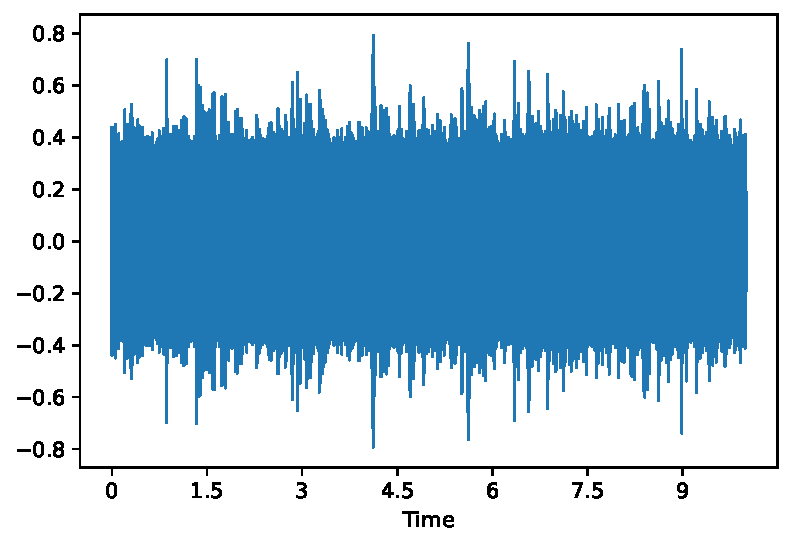
\includegraphics[width=\textwidth]{../images/audio/birds.wave.birdvox.pdf}
            \label{fig:birds.wave.birdvox}
        \end{subfigure}
        \hfill
        \begin{subfigure}[b]{0.45\textwidth}
            \centering
            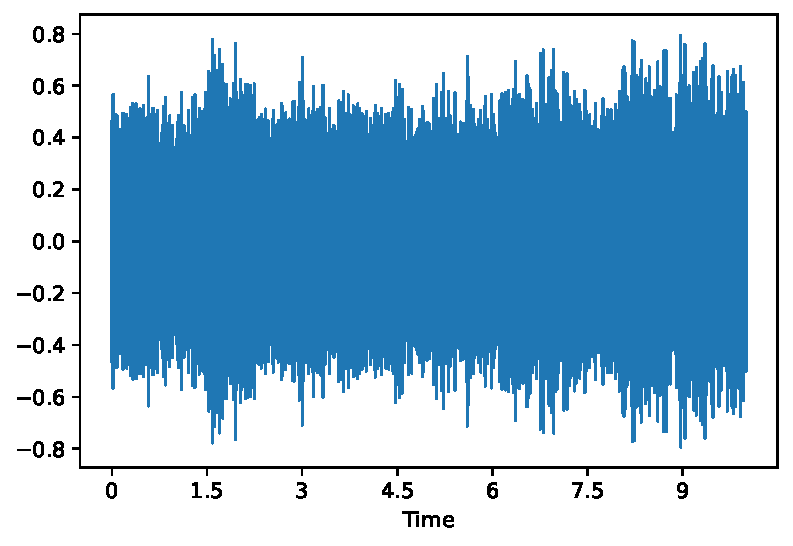
\includegraphics[width=\textwidth]{../images/audio/nobirds.wave.birdvox.pdf}
            \label{fig:nobirds.wave.birdvox}
        \end{subfigure}

        \vspace{-0.7cm}

        \begin{subfigure}[b]{0.45\textwidth}
            \centering
            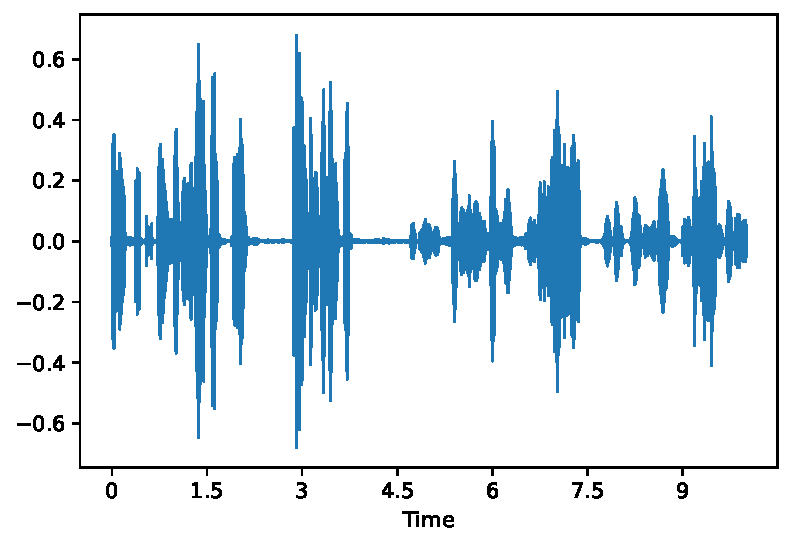
\includegraphics[width=\textwidth]{../images/audio/birds.wave.ff1010.pdf}
            \caption{Enregistrement contenant des oiseaux}
            \label{fig:birds.wave.ff1010}
        \end{subfigure}
        \hfill
        \begin{subfigure}[b]{0.45\textwidth}
            \centering
            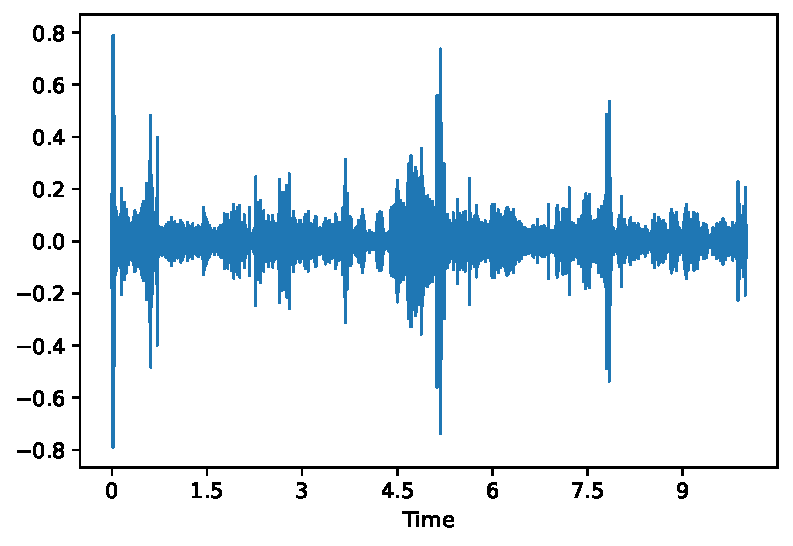
\includegraphics[width=\textwidth]{../images/audio/nobirds.wave.ff1010.pdf}
            \caption{Enregistrement ne contenant pas d'oiseaux}
            \label{fig:nobirds.wave.ff1010}
        \end{subfigure}
    \end{figure}

\end{frame}

% \begin{frame}{Représentation temporelle (forme d'onde)}

%     \begin{block}{Avantages}
%         \begin{itemize}
%             \item Visualisation intuitive du signal audio. % permettant de détecter les changements rapides ou lents dans l'amplitude du son.
%             \item Identifier les moments de silence ou de faible amplitude, ainsi que les pics et les moments d'intensité sonore élevée.
%             \item Repérer des motifs ou des caractéristiques spécifiques dans le signal audio.
%         \end{itemize}
%     \end{block}

%     \begin{alertblock}{Inconvénients}
%         \begin{itemize}
%             \item Pas d'informations détaillées sur la nature exacte des composantes fréquentielles du son.
%             \item Ne permet pas d'identifier précisément les différentes sources sonores présentes dans le signal.
%             \item Limité par la résolution temporelle de l'affichage. % ce qui peut rendre difficile la détection de variations très rapides ou de détails fins dans le signal audio.
%         \end{itemize}
%     \end{alertblock}

% \end{frame}

% \begin{frame}{Représentation spectrale}
%     Nécessité de se tourner vers des représentations \textbf{spectrales}.

%     \begin{block}{Avantages}
%         \begin{itemize}
%             \item Visualiser des composantes fréquentielles du signal audio. % permettant de détecter les changements rapides ou lents dans l'amplitude du son.
%             \item Identifier les changements de fréquence, les harmoniques et les caractéristiques spectrales spécifiques.
%             \item Utile pour la \textbf{détection d'événements sonores}, la classification d'instruments, l'analyse musicale...
%         \end{itemize}
%     \end{block}

%     \begin{alertblock}{Inconvénients}
%         \begin{itemize}
%             % \item Pas d'informations détaillées sur les variations temporelles du signal audio.
%             \item Peut nécessiter une résolution temporelle plus fine pour représenter les variations rapides dans le signal.
%             \item Processus parfois irréversible...
%         \end{itemize}
%     \end{alertblock}

% \end{frame}

\begin{frame}{Représentation spectrale}
    Mais il existe plusieurs représentations... laquelle choisir ?

    \begin{exampleblock}{Les plus communes...}
        \begin{itemize}
            \item Spectrogramme ?
            \item Chromagramme ?
            \item Cepstre ?
        \end{itemize}
    \end{exampleblock}

    $\Rightarrow$ Dans tous les cas : Fourier !
\end{frame}


% \begin{frame}{Représentation spectrale : Chromagramme}
%     Mais il existe plusieurs représentations... laquelle choisir ?

%     \begin{block}{Chromagramme}

%         \begin{itemize}
%             \item Représentation temps/notes de musique.
%             \item Met l'accent sur les informations tonales et harmoniques d'un signal audio.
%             \item Largement utilisé dans des applications telles que la transcription musicale automatique, la reconnaissance des accords et l'analyse comparative de morceaux de musique.
%         \end{itemize}

%     \end{block}

%     $\Rightarrow$ Représentation peu utilisée dans la littérature pour notre défi.

% \end{frame}

\begin{frame}{Représentation spectrale : Chromagramme}

    Sur des données issues de BirdVox...

    \begin{figure}[ht]
        \centering
        \begin{subfigure}[b]{0.45\textwidth}
            \centering
            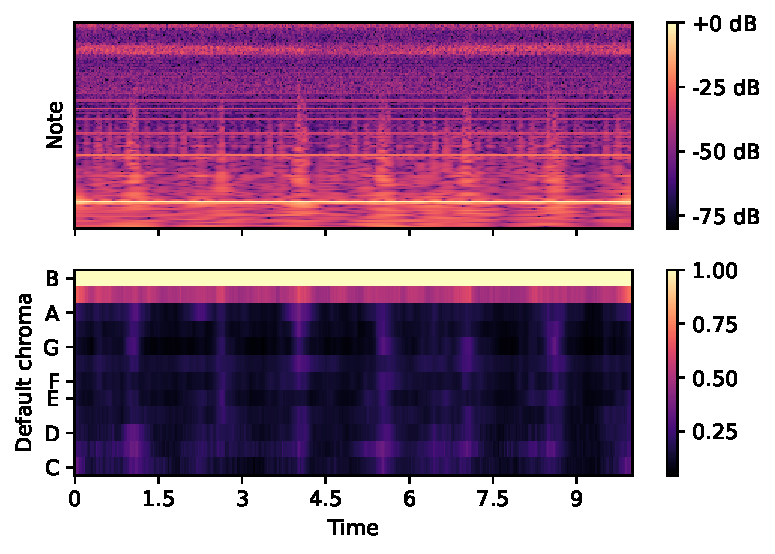
\includegraphics[width=\textwidth]{../images/audio/birds.chromagram.birdvox.pdf}
            \caption{Enregistrement contenant des oiseaux}
            \label{fig:birds.chromagram.birdvox}
        \end{subfigure}
        \hfill
        \begin{subfigure}[b]{0.45\textwidth}
            \centering
            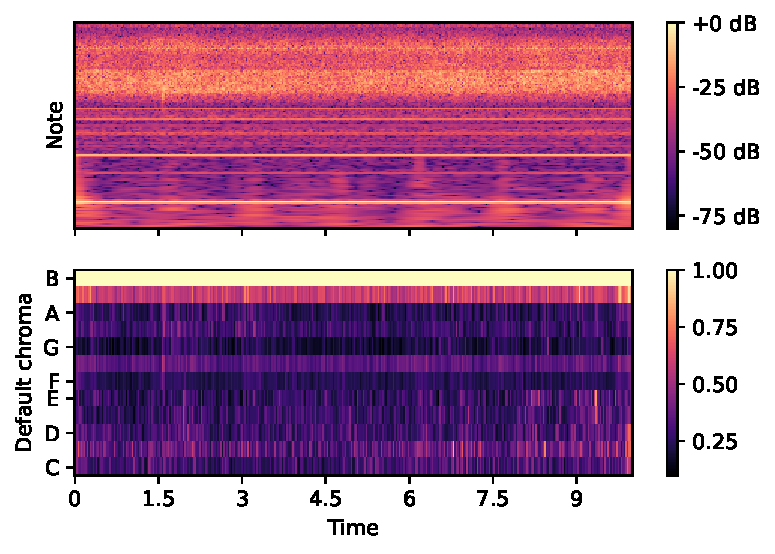
\includegraphics[width=\textwidth]{../images/audio/nobirds.chromagram.birdvox.pdf}
            \caption{Enregistrement ne contenant pas d'oiseaux}
            \label{fig:nobirds.chromagram.birdvox}
        \end{subfigure}
    \end{figure}

\end{frame}

\begin{frame}{Représentation spectrale : Chromagramme}

    Sur des données issues de Freefield...

    \begin{figure}[ht]
        \centering
        \begin{subfigure}[b]{0.45\textwidth}
            \centering
            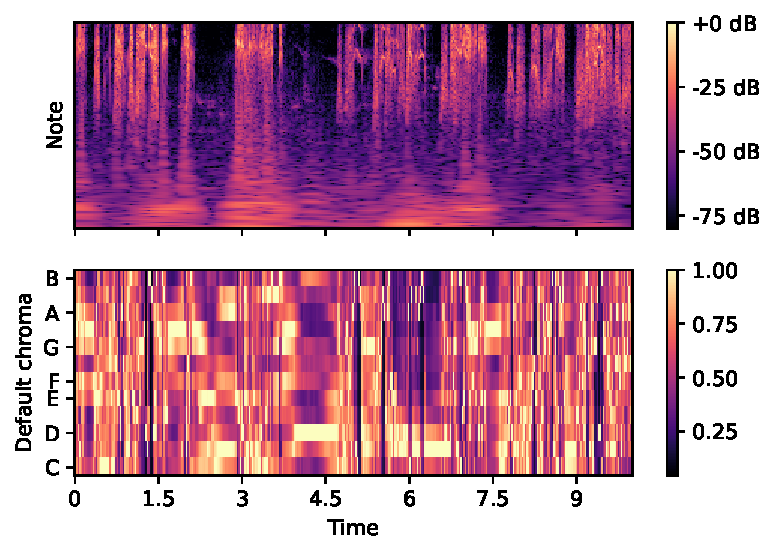
\includegraphics[width=\textwidth]{../images/audio/birds.chromagram.ff1010.pdf}
            \caption{Enregistrement contenant des oiseaux}
            \label{fig:birds.chromagram.ff1010}
        \end{subfigure}
        \hfill
        \begin{subfigure}[b]{0.45\textwidth}
            \centering
            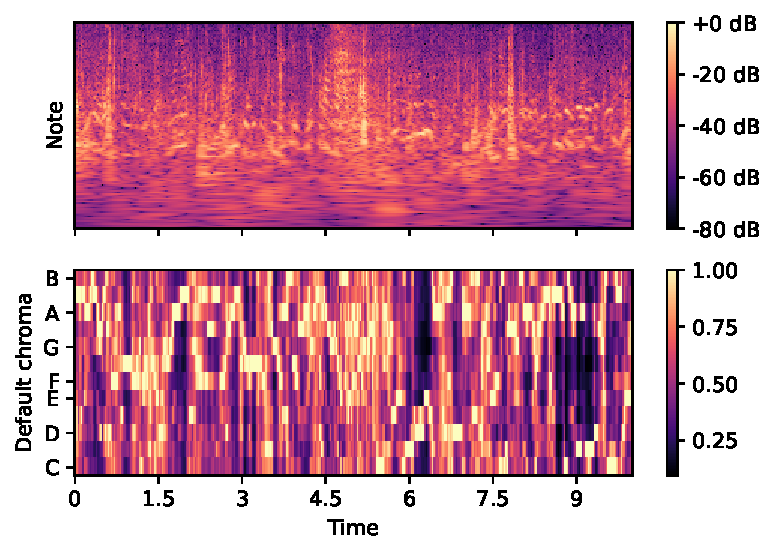
\includegraphics[width=\textwidth]{../images/audio/nobirds.chromagram.ff1010.pdf}
            \caption{Enregistrement ne contenant pas d'oiseaux}
            \label{fig:nobirds.chromagram.ff1010}
        \end{subfigure}
    \end{figure}


\end{frame}

% \begin{frame}{Représentation spectrale : Cepstre}
%     Mais il existe plusieurs représentations... laquelle choisir ?

%     \begin{block}{Cepstre}

%         \begin{itemize}
%             \item Met l'accent sur l'étude structures périodiques temporelles des caractéristiques spectrales d'un signal audio.
%             \item Fournit des informations sur les enveloppes spectrales et les variations dans le domaine fréquentiel du signal.
%             \item Utile pour l'analyse des formants vocaux, la détection des harmoniques, la reconnaissance de la parole et d'autres applications liées aux caractéristiques temporelles du signal audio.
%             \item Réversible !
%         \end{itemize}

%     \end{block}

%     $\Rightarrow$ Représentation \textbf{intéressante} pour notre défi et utilisée dans la littérature. Est-ce la plus \textbf{pertinente} ?

% \end{frame}

\begin{frame}{Représentation spectrale : Cepstre}

    Sur des données issues de BirdVox...

    \begin{figure}[ht]
        \centering
        \begin{subfigure}[b]{0.45\textwidth}
            \centering
            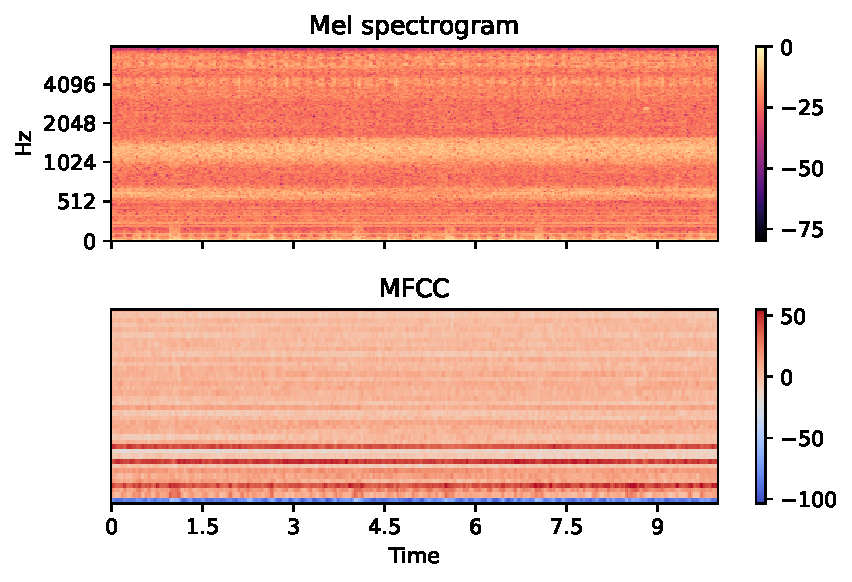
\includegraphics[width=\textwidth]{../images/audio/birds.mfcc.birdvox.pdf}
            \caption{Enregistrement contenant des oiseaux}
            \label{fig:birds.mfcc.birdvox}
        \end{subfigure}
        \hfill
        \begin{subfigure}[b]{0.45\textwidth}
            \centering
            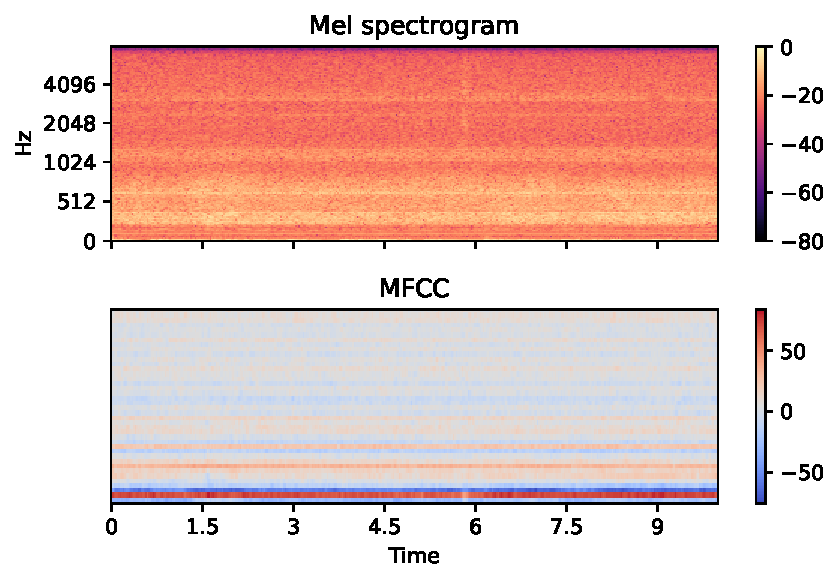
\includegraphics[width=\textwidth]{../images/audio/nobirds.mfcc.birdvox.pdf}
            \caption{Enregistrement ne contenant pas d'oiseaux}
            \label{fig:nobirds.mfcc.birdvox}
        \end{subfigure}
    \end{figure}

\end{frame}

\begin{frame}{Représentation spectrale : Cepstre}

    Sur des données issues de Freefield...

    \begin{figure}[ht]
        \centering
        \begin{subfigure}[b]{0.45\textwidth}
            \centering
            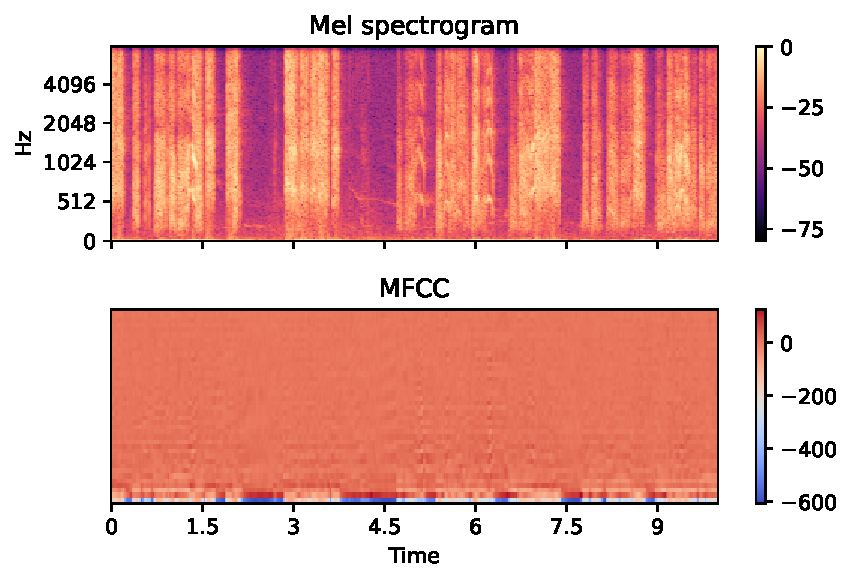
\includegraphics[width=\textwidth]{../images/audio/birds.mfcc.ff1010.pdf}
            \caption{Enregistrement contenant des oiseaux}
            \label{fig:birds.mfcc.ff1010}
        \end{subfigure}
        \hfill
        \begin{subfigure}[b]{0.45\textwidth}
            \centering
            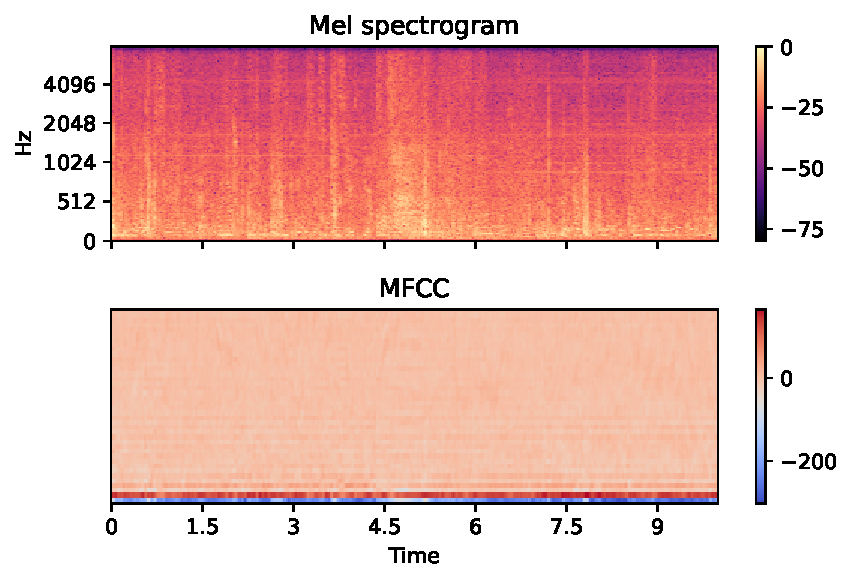
\includegraphics[width=\textwidth]{../images/audio/nobirds.mfcc.ff1010.pdf}
            \caption{Enregistrement ne contenant pas d'oiseaux}
            \label{fig:nobirds.mfcc.ff1010}
        \end{subfigure}
    \end{figure}

\end{frame}

% \begin{frame}{Représentation spectrale : Spectrogramme}
%     Mais il existe plusieurs représentations... laquelle choisir ?

%     \begin{block}{Spectrogramme}

%         \begin{itemize}
%             \item Représentation temps/fréquence.
%             \item Met l'accent sur la répartition spectrale de l'énergie ou de la puissance du signal audio.
%             \item Utile pour observer les changements de fréquences, les harmoniques, les transitions tonales et les événements sonores dans le temps.
%             \item Possibilité de passer en 3D : temps/fréquence/amplitude.
%         \end{itemize}

%     \end{block}

%     $\Rightarrow$ Représentation \textbf{la plus utilisée} dans la littérature.

% \end{frame}

\begin{frame}{Représentation spectrale : Spectrogramme}

    Sur des données issues de BirdVox...

    \begin{figure}[ht]
        \centering
        \begin{subfigure}[b]{0.45\textwidth}
            \centering
            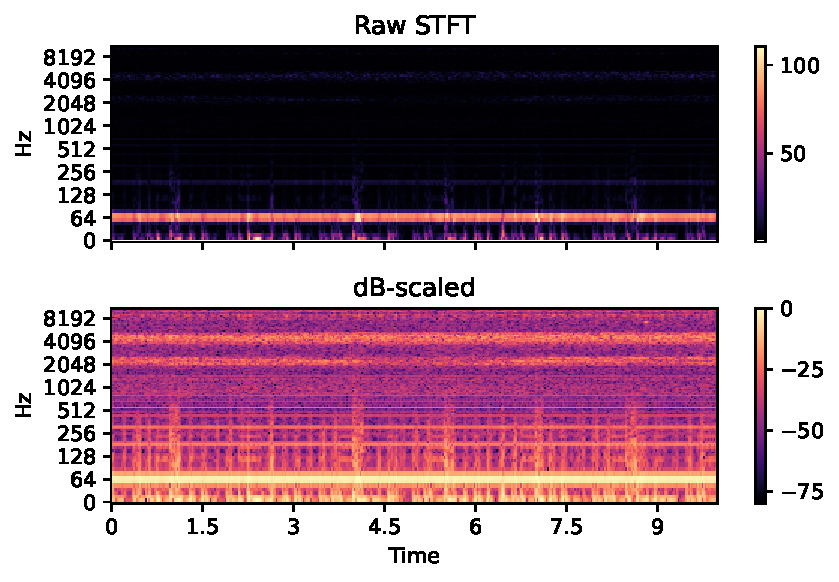
\includegraphics[width=\textwidth]{../images/audio/birds.spectrogram.birdvox.pdf}
            \caption{Enregistrement contenant des oiseaux}
            \label{fig:birds.spectrogram.birdvox}
        \end{subfigure}
        \hfill
        \begin{subfigure}[b]{0.45\textwidth}
            \centering
            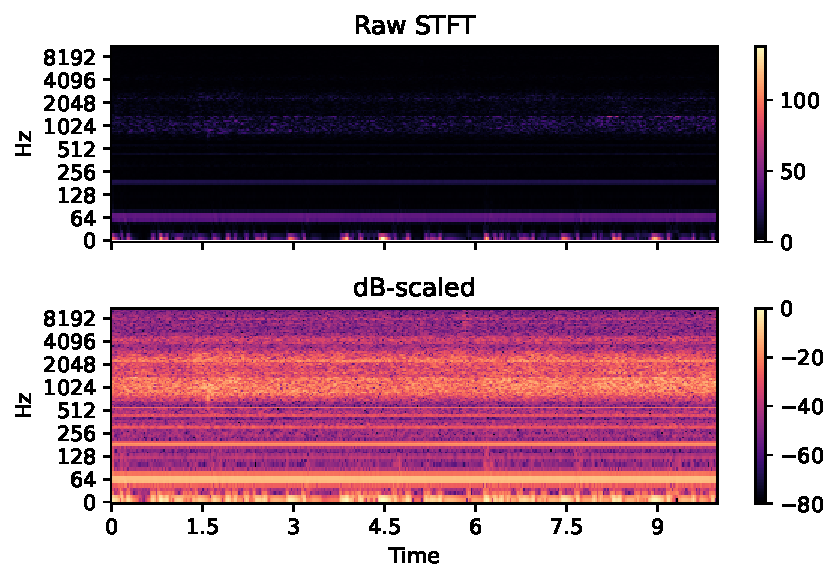
\includegraphics[width=\textwidth]{../images/audio/nobirds.spectrogram.birdvox.pdf}
            \caption{Enregistrement ne contenant pas d'oiseaux}
            \label{fig:nobirds.spectrogram.birdvox}
        \end{subfigure}
    \end{figure}

\end{frame}

\begin{frame}{Représentation spectrale : Spectrogramme}

    Sur des données issues de Freefield...

    \begin{figure}[ht]
        \centering
        \begin{subfigure}[b]{0.45\textwidth}
            \centering
            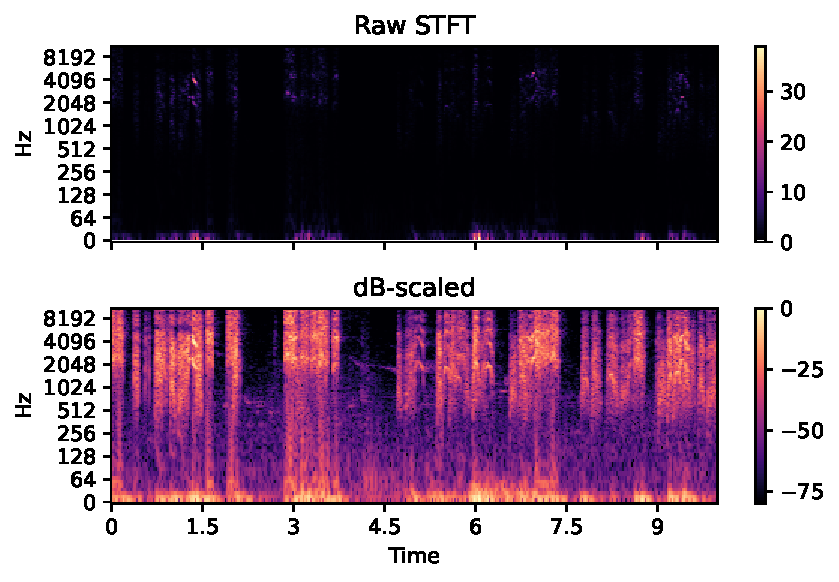
\includegraphics[width=\textwidth]{../images/audio/birds.spectrogram.ff1010.pdf}
            \caption{Enregistrement contenant des oiseaux}
            \label{fig:birds.spectrogram.ff1010}
        \end{subfigure}
        \hfill
        \begin{subfigure}[b]{0.45\textwidth}
            \centering
            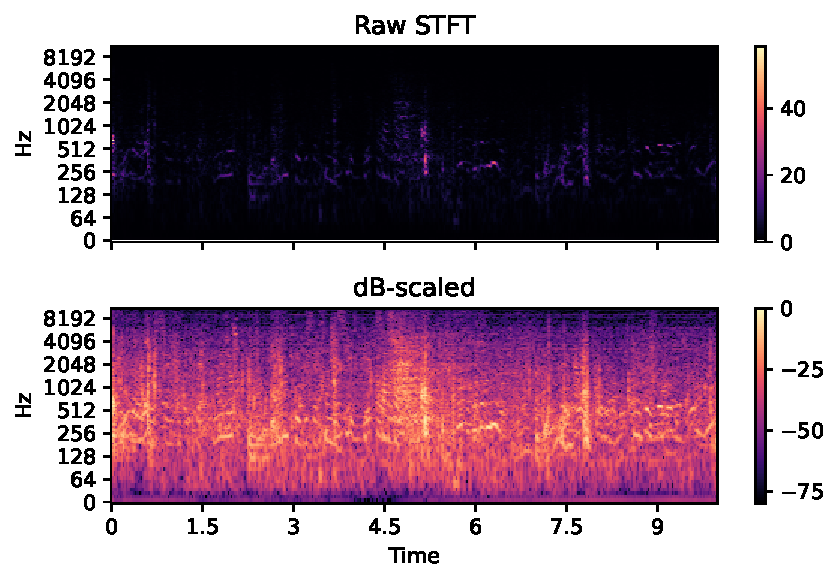
\includegraphics[width=\textwidth]{../images/audio/nobirds.spectrogram.ff1010.pdf}
            \caption{Enregistrement ne contenant pas d'oiseaux}
            \label{fig:nobirds.spectrogram.ff1010}
        \end{subfigure}
    \end{figure}

\end{frame}

\begin{frame}{Et maintenant ?}
    En plus de transformer la représentation, il y a d'autres façons de pré-traiter les données en traitement du signal. Entre autres :

    \begin{block}{Pré-traitements}
        \begin{itemize}
            \item Normalisation
            \item Réduction de bruit
            \item Élimination des artefacts et des imperfections
            \item Augmentation de données
            \item Modification temporelle et fréquentielle
            \item Détection et suppression de "mots-clés"
        \end{itemize}
    \end{block}

    Beaucoup de pistes : tout explorer est \textbf{chronophage} mais serait intéressant, d'un point de vue théorique et fondamental.

\end{frame}

% \begin{frame}{Pré-traitements}

%     \begin{exampleblock}{Normalisation}
%         \begin{itemize}
%             \item Normalisation de l'amplitude
%             \item Compression dynamique
%             \item Ajustement des niveaux de volume
%         \end{itemize}
%     \end{exampleblock}

%     \begin{exampleblock}{Noise reduction}
%         \begin{itemize}
%             \item Filtrage adaptatif
%             \item Soustraction spectrale
%             \item Réduction de bruit par seuillage
%             \item Réduction de bruit par modélisation statistique
%         \end{itemize}
%     \end{exampleblock}

% \end{frame}

% \begin{frame}{Pré-traitements}

%     \begin{exampleblock}{Élimination des artefacts et des imperfections}
%         \begin{itemize}
%             \item Élimination des silences et des clics
%             \item Détection et suppression des artefacts
%             \item Correction des distorsions
%             \item Suppression de la réverbération
%         \end{itemize}
%     \end{exampleblock}

%     \begin{exampleblock}{Data augmentation}
%         \begin{itemize}
%             \item Variations de vitesse et de tonalité
%             \item Mixage de sources audio
%             \item Perturbations et déformations synthétiques
%             \item \textbf{Chunking}
%         \end{itemize}
%     \end{exampleblock}

% \end{frame}

% \begin{frame}{Pré-traitements}

%     \begin{exampleblock}{Modification temporelle et fréquentielle}
%         \begin{itemize}
%             \item Normalisation temporelle (time-stretching)
%             \item Modification de la vitesse (time-scaling)
%             \item Modification de la tonalité (pitch-shifting)
%             \item Time-domain resampling
%         \end{itemize}
%     \end{exampleblock}

%     \begin{exampleblock}{Détection et suppression de "mots-clés"}
%         \begin{itemize}
%             \item Séparation de parole et de musique
%             \item Détection et suppression de mots-clés spécifiques
%         \end{itemize}
%     \end{exampleblock}

%     Liste non-exhaustive... mais le pré-traitement n'est qu'une première étape, son efficacité dépendra également du modèle d'apprentissage derrière !

% \end{frame}

\begin{frame}{Quels pré-traitements explorer ?}

    Nous avons choisi d'explorer \textbf{3 approches} différentes pour le pré-traitement.

    \begin{block}{Approches choisies}
        \begin{itemize}
            \item Spectrogramme + Suppression du bruit + Découpage en chunks.
            \item Spectrogramme + Supression du bruit.
            \item Mel-Spectrogramme.
        \end{itemize}
    \end{block}

\end{frame}

\begin{frame}{Première approche}

    \begin{block}{\citetitle{sprengelAudioBasedBird2016} \cite{sprengelAudioBasedBird2016}}
        Utilise des opérations d'érosion et de dilation puis divise les audios en chunks de 2 secondes.
        \begin{itemize}
            \item Calcul du spectrogramme, estime le bruit à partir du calcul des médianes.
            \item Extraction du masque binaire.
            \item Modifie la forme des objets binaires par érosion et dilatation.
            \item Division en chunks.
        \end{itemize}
    \end{block}

\end{frame}

\begin{frame}{Première approche}

    \begin{figure}[ht]
        \centering
        \begin{subfigure}[b]{0.45\textwidth}
            \centering
            \caption*{Spectrogramme original}
            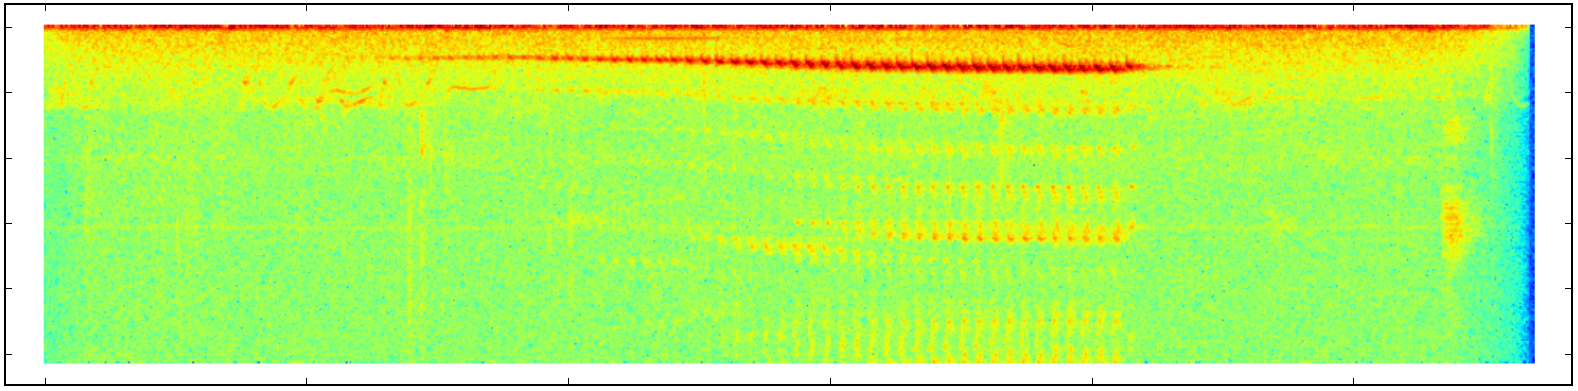
\includegraphics[width=\textwidth]{../images/chunks.original_spectrogram.png}
            \label{fig:chunks.original_spectrogram}
        \end{subfigure}
        \hfill
        \begin{subfigure}[b]{0.45\textwidth}
            \centering
            \caption*{Pixels sélectionnés après érosion}
            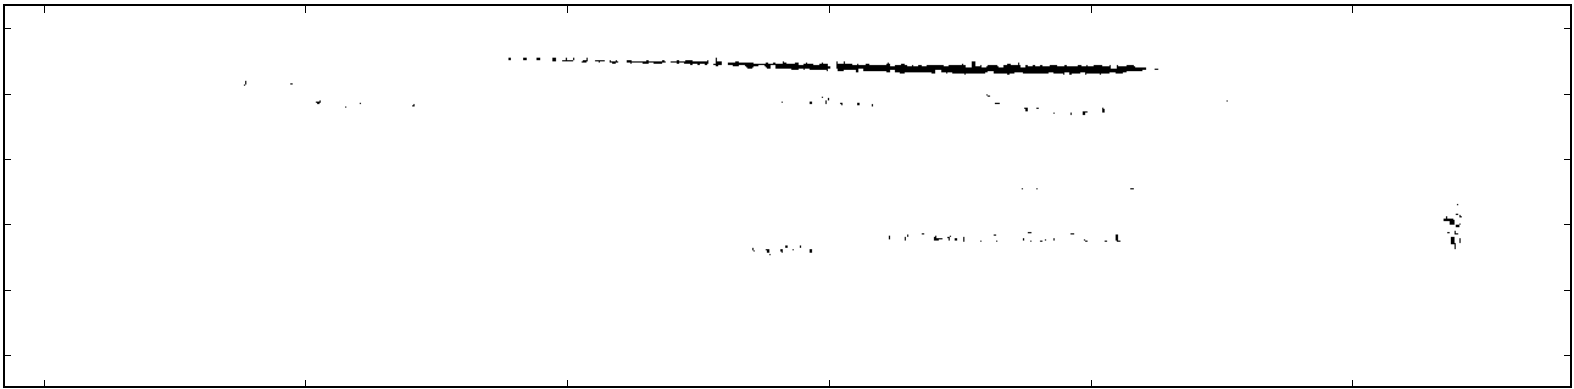
\includegraphics[width=\textwidth]{../images/chunks.selected_pixels_after_erosion.png}
            \label{fig:chunks.selected_pixels_after_erosion}
        \end{subfigure}

        \vspace{0.5cm}

        \begin{subfigure}[b]{0.45\textwidth}
            \centering
            \caption*{Pixels sélectionnés}
            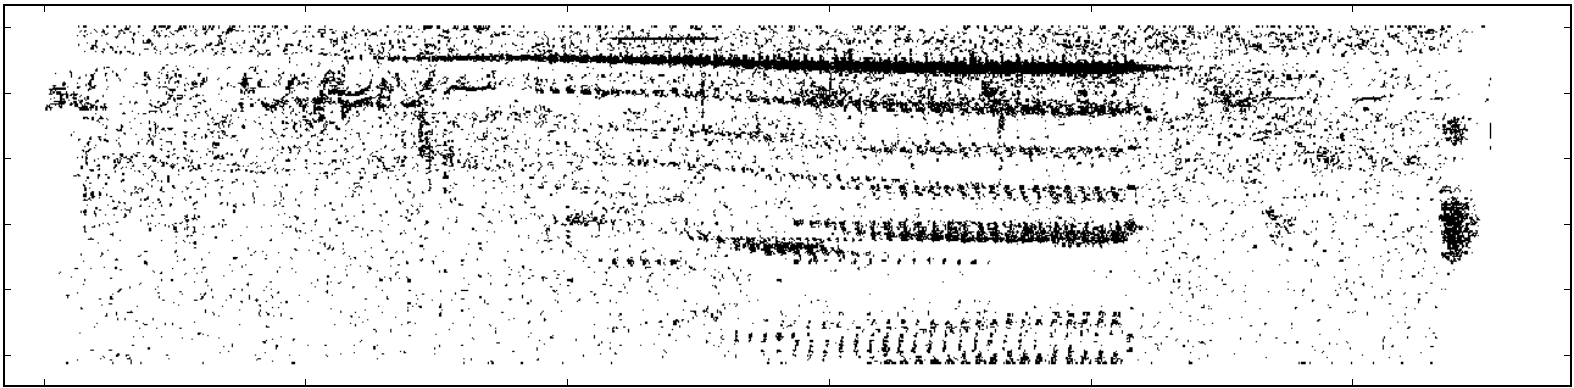
\includegraphics[width=\textwidth]{../images/chunks.selected_pixels.png}
            \label{fig:chunks.selected_columns}
        \end{subfigure}
        \hfill
        \begin{subfigure}[b]{0.45\textwidth}
            \centering
            \caption*{Pixels sélectionnés après érosion et dilatation}
            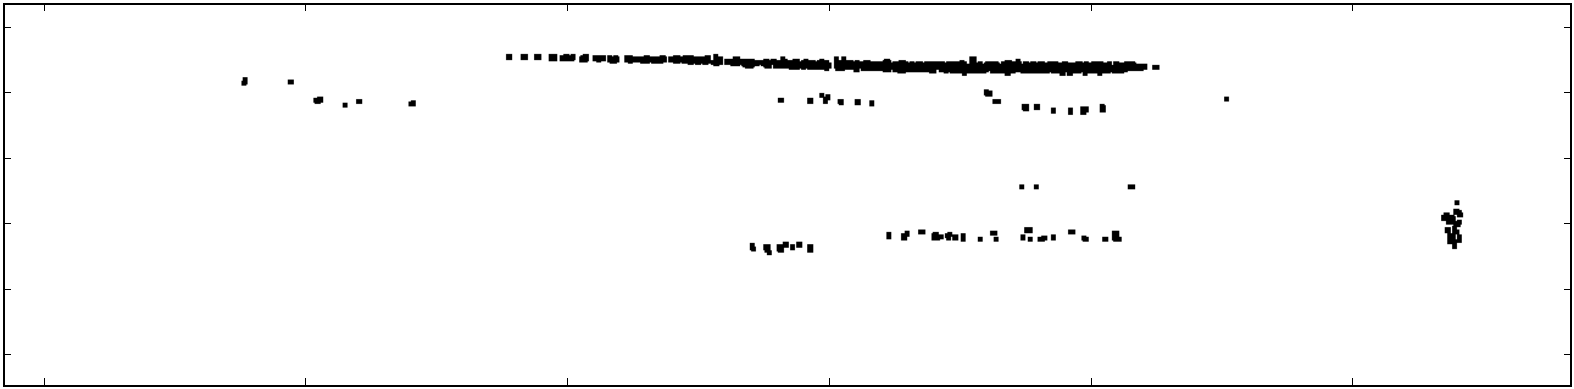
\includegraphics[width=\textwidth]{../images/chunks.selected_pixels_erosion_dilation.png}
            \label{fig:chunks.selected_pixels_erosion_dilation}
        \end{subfigure}
    \end{figure}


\end{frame}

\begin{frame}{Deuxième approche}

    \begin{block}{\citetitle{sprengelAudioBasedBird2016} \cite{sprengelAudioBasedBird2016}}
        Dans cette approche, nous nous concentrerons sur la fonction \texttt{reduce\_noise} de la bibliothèque \texttt{noisereduce}, qui est une technique couramment utilisée pour supprimer le bruit des enregistrements audio.

        \begin{itemize}
            \item Préservation du signal. 
            \item Robustesse.
            \item Adaptabilité.
        \end{itemize}
    \end{block}

% $\Rightarrow$ Préservation du signal. \\
% $\Rightarrow$ Robustesse. \\
% $\Rightarrow$ Adaptabilité.

\end{frame}

\begin{frame}{Deuxième approche}

    \begin{figure}[ht]
        \centering
        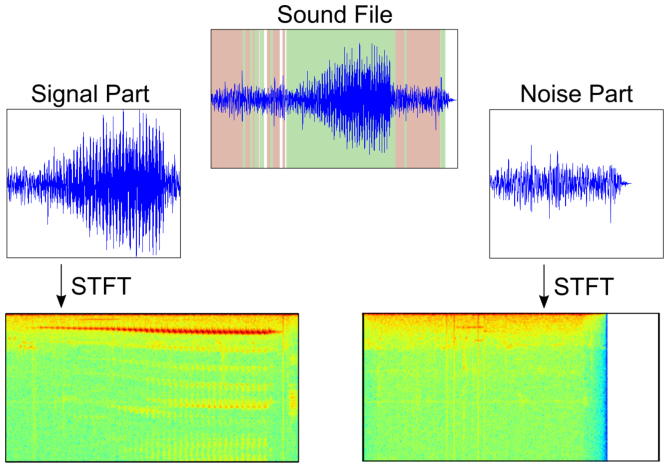
\includegraphics[width=\textwidth,height=0.8\textheight,keepaspectratio]{../images/noisereduce.pdf}
        \caption{Séparation du signal et de la partie bruitée d'un audio}
        \label{fig:noisereduce}
    \end{figure}

\end{frame}

\section{Modélisation} \subsection{}

\begin{frame}{État de l'art - SVM}

    Ce qui se faisait... et se fait encore : modèles "classiques" de \textit{machine learning}.

    Prix du jury du challenge 2016/2017 :

    \begin{exampleblock}{\citetitle{thakurRapidBirdActivity2017} \cite{thakurRapidBirdActivity2017}}

        \begin{itemize}
            \item SVM (+ GMM).
            \item Kernels "dynamiques" : probabilistic sequence kernel.
            \item Pré-traitements : MFCC, cepstral normalisation, short-time Gaussianization.
        \end{itemize}

        $\Rightarrow$ Faible complexité calculatoire par rapport à des modèles \textit{deep} mais moins performant (75.2~\%).

    \end{exampleblock}

\end{frame}


\begin{frame}{État de l'art - CNN}

    Ce qui marche le mieux : les réseaux de neurones.

    Grand gagnant du challenge 2016/2017 :

    \begin{exampleblock}{\citetitle{grillTwoConvolutionalNeural2017} \cite{grillTwoConvolutionalNeural2017}}

        \begin{itemize}
            \item Architecture CNN classique.
            \item Pré-traitements : silence/noise trimming + data augmentation.
            \item PCA + Agglomerative Clustering à partir des features du spectrogramme (moyenne, écart-type, 1-percentile, 99-percentile).
            \item Adaptation de domaine : pseudo-labeling.
            \item Ensembling : model averaging.
        \end{itemize}

    \end{exampleblock}

\end{frame}

\begin{frame}{État de l'art - CRNN}

    Ce qui marche le mieux : les réseaux de neurones.

    Prix du jury du challenge 2016/2017 :

    \begin{exampleblock}{\citetitle{cakirConvolutionalRecurrentNeural2017a} \cite{cakirConvolutionalRecurrentNeural2017a}}

        \begin{itemize}
            \item Modèle \og~hybride~\fg : CNN + RNN = CRNN.
            \item Résultats \textit{très} proches du modèle le plus performant (88.5~\% vs 88.7~\%).
            \item Bien moins computationally intensive que le modèle le plus performant.
            \item Pas de data augmentation, d'adaptation de domaine ou d'ensembling.
        \end{itemize}

    \end{exampleblock}

\end{frame}

\begin{frame}{Quelles modélisations explorer ?}

    Nous avons choisi d'explorer \textbf{4 approches} différentes pour la modélisation.

    \begin{block}{Approches de modélisation}
        \begin{itemize}
            \item CNN
            \item RNN
            \item SVM
            \item CRNN
        \end{itemize}
    \end{block}



\end{frame}

\begin{frame}{Pourquoi un CNN ? }

    \begin{block}{Atouts}
        \begin{itemize}
            \item Représentation spatio-temporelle.
            \item Hiérarchie des caractéristiques.
            \item Invariance aux translations.
            \item Capacité à gérer des données de grande taille.
            \item Apprentissage de représentations discriminantes.
        \end{itemize}
    \end{block}

    \begin{figure}
        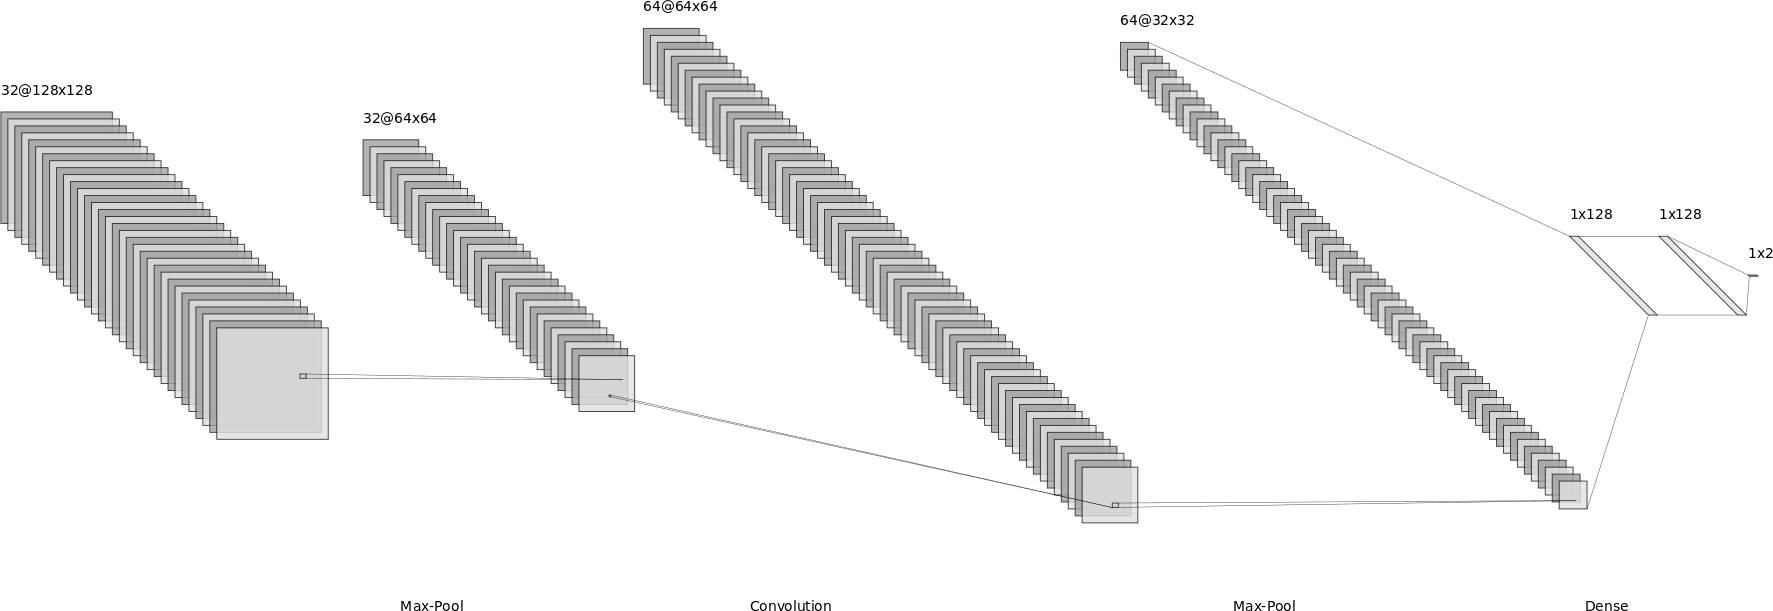
\includegraphics[width=\textwidth,keepaspectratio]{../images/models/CNN.architecture.png}
        \caption{Architecture CNN proposée pour la détection d'oiseaux}
        \label{fig:CNN.architecture.birds}
    \end{figure}

\end{frame}

\begin{frame}{Pourquoi un RNN ?}

    \begin{block}{Atouts}
        \begin{itemize}
            \item Gestion des séquences temporelles.
            \item Capture des dépendances à long terme.
            \item Traitement de séquences de longueur variable.
            \item Adaptabilité aux différentes fréquences d'échantillonnage.
        \end{itemize}
    \end{block}

    \begin{figure}
        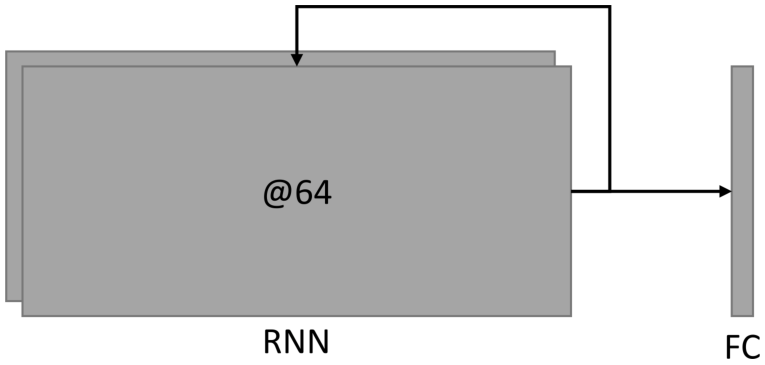
\includegraphics[height=0.35\textheight,keepaspectratio]{../images/models/RNN.architecture.pdf}
        \caption{Architecture RNN proposée pour la détection d'oiseaux}
        \label{fig:RNN.architecture.birds}
    \end{figure}

\end{frame}

\begin{frame}{Quelles expérimentations ?}
    
    \begin{block}{Pour le CNN...}
        \begin{itemize}
            \item Ajouter une couche dense supplémentaires ?
            \item Jouer avec la couche de pooling (par exemple, average pooling au lieu de max pooling) ?
        \end{itemize}
    \end{block}

    \begin{block}{Pour le RNN...}
        \begin{itemize}
            \item Ajouter une couche de sortie supplémentaire avec une fonction d'activation (ou non) ReLU ?
            \item GRU ? LSTM ? Bi-LSTM ?
        \end{itemize}
    \end{block}

\end{frame}

\begin{frame}{Pourquoi ne pas essayer un SVM ?}

    Après tout...

    \begin{block}{Atouts}
        \begin{itemize}
            \item Gestions des espaces de grande dimension.
            \item Contrôle du sur-ajustement.
            \item Flexibilité du choix de la fonction de noyau.
            \item Efficacité en présence de données déséquilibrées.
        \end{itemize}
    \end{block}

\end{frame}

\begin{frame}{CRNN}

    \begin{block}{\cite{cakirConvolutionalRecurrentNeural2017a}}

        \begin{itemize}
            \item Modèle développé dans le cadre de la détection de sons polyphoniques, c'est-à-dire la détection de plusieurs événements sonores se chevauchant.
            \item Postulat que CNN et RNN sont deux méthodes complémentaires.
        \end{itemize}

    \end{block}

    \begin{alertblock}{Mais...}

        ...modèle toujours d'actualité ?

    \end{alertblock}

\end{frame}

\begin{frame}{CRNN - Ce n'est pas une révolution...}

    Pas nouveau... mais diffèrent des architectures CRNN précédentes :

    \begin{exampleblock}{\cite{cakirConvolutionalRecurrentNeural2017a}}

        \begin{itemize}
            \item Aucune utilisation de couche linéaire après le CNN ou RNN.
            \item Kernels de convolution plus petits.
            \item Jusqu'à 4 couches de convolution, 3 couche de récurrence.
            \item GRU au lieu de LSTM.
            \item Séquences plus longues.
            \item Utilisation optionnelle d'une couche supplémentaire de \textit{temporal pooling} à la sortie du RNN.
        \end{itemize}

    \end{exampleblock}

    $\Rightarrow$ Surpasse les GMM, FNN, CNN et RNN classiques.

\end{frame}

\begin{frame}{CRNN - Architecture}

    \begin{figure}[ht]
        \centering
        \begin{subfigure}[b]{0.45\textwidth}
            \centering
            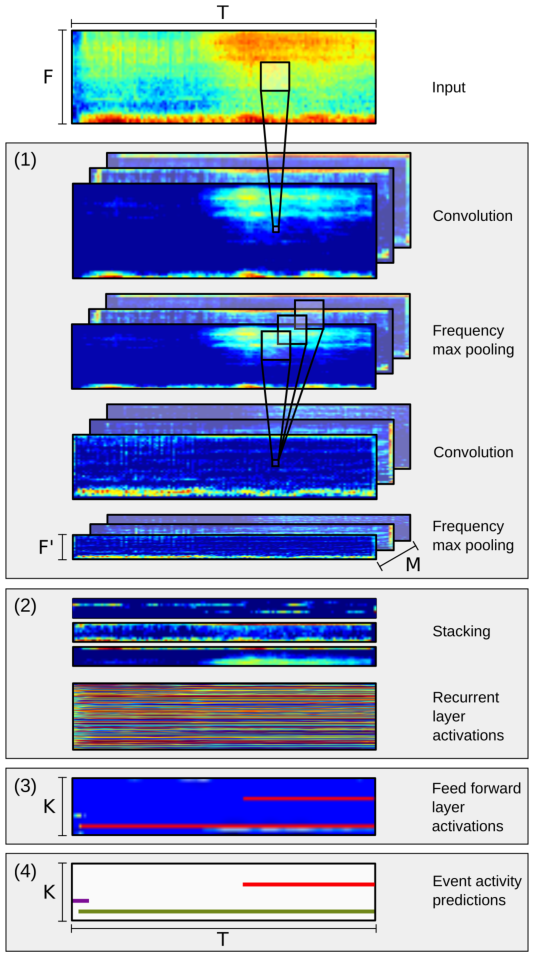
\includegraphics[width=\textwidth,height=0.8\textheight,keepaspectratio]{../images/models/CRNN.architecture.generic.pdf}
            \caption{Architecture générique du CRNN\\~}
            \label{fig:CRNN.architecture.generic}
        \end{subfigure}
        \hfill
        \begin{subfigure}[b]{0.45\textwidth}
            \centering
            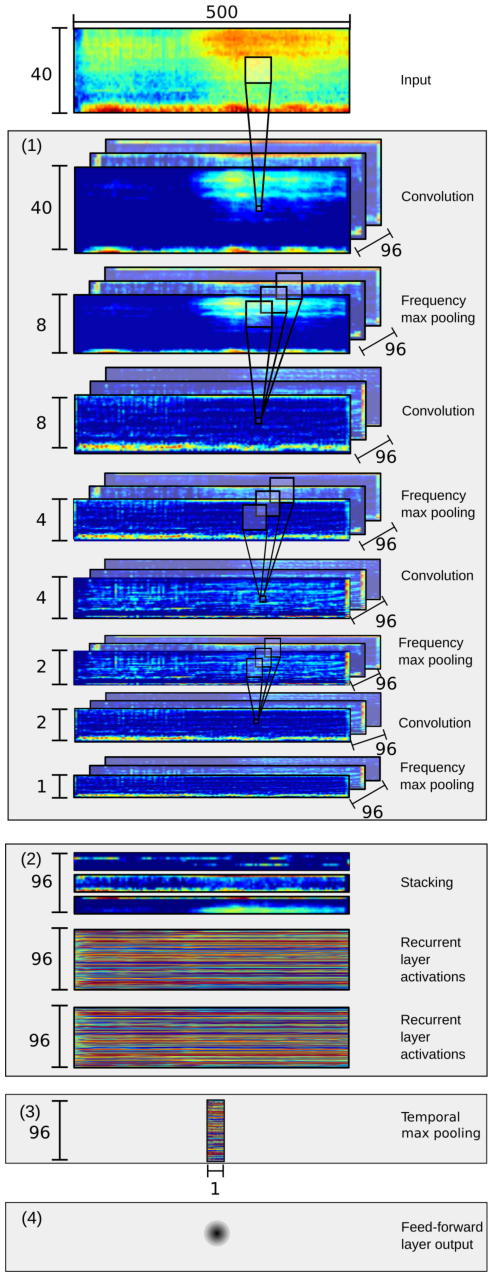
\includegraphics[width=\textwidth,height=0.8\textheight,keepaspectratio]{../images/models/CRNN.architecture.birds.pdf}
            \caption{Architecture CRNN proposée pour la détection d'oiseaux}
            \label{fig:CRNN.architecture.birds}
        \end{subfigure}
    \end{figure}

\end{frame}

\begin{frame}{CRNN - Que peut-on en dire ?}

    On travaille \textbf{sur des \textit{images}} (spectrogrammes), \textbf{dans le temps} $\Rightarrow$ le modèle est entièrement fondé, mais pouvons-nous apporter des améliorations ?

    \begin{block}{La couche récurrente : GRU ?}
        GRU se "limite" à capturer des dépendances à court terme.

        \begin{itemize}
            \item En a-t-on \textit{réellement} besoin ?
            \item Un RNN suffirait-il ?
            \item Un LSTM serait-il plus apte à capturer des informations ?
            \item Méthodes plus "modernes"...?
        \end{itemize}

    \end{block}

\end{frame}

\begin{frame}{CRNN - Que peut-on en dire ?}

    On travaille \textbf{sur des \textit{images}} (spectrogrammes), \textbf{dans le temps} $\Rightarrow$ le modèle est entièrement fondé, mais pouvons-nous apporter des améliorations ?

    \begin{block}{La couche de \textit{temporal pooling}}
        But : réduire la dimension temporelle tout en préservant les features les plus importantes.

        \begin{itemize}
            \item En a-t-on \textit{réellement} besoin ?
            \item Pourquoi ne pas regarder directement sur la sortie temporelle ?
            \item Méthodes plus "modernes"...?
        \end{itemize}
    \end{block}

\end{frame}

\begin{frame}{CRNN - Méthodes plus modernes ?}

    \begin{figure}[ht]
        \centering
        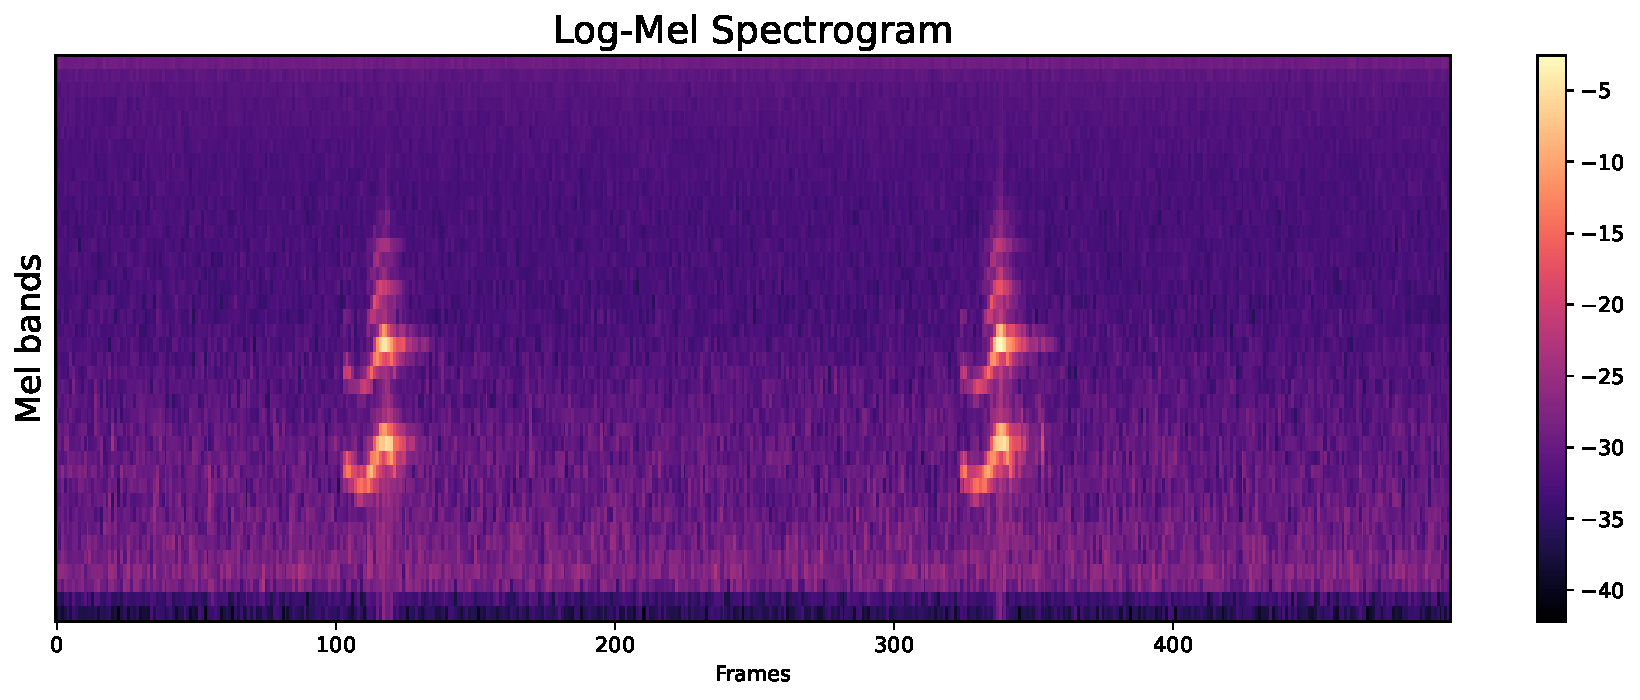
\includegraphics[width=\textwidth]{../images/audio/birds.melspectrogram.ff1010.pdf}
        \caption{Log mel-band energies d'un son contenant un oiseau}
        \label{fig:birds.melspectrogram.ff1010}
    \end{figure}

\end{frame}

\begin{frame}{CRNN - Attention you say?}

    La révolution de l'\textbf{attention}.

    \begin{block}{\citetitle{attentionIsAllYouNeed} \cite{attentionIsAllYouNeed}}
        Se concentrer sur des parties spécifiques d'une séquence, afin de capturer des relations à longue portée.

        \begin{itemize}
            \item Des Transformers à la place d'une couche récurrente ?
            \item De l'attention \textit{pure} (soft ? hard ?) à la place d'une couche de pooling temporelle ?
        \end{itemize}
    \end{block}

\end{frame}

\section{Expérimentations} \subsection{}

\begin{frame}{Méthode d'évaluation}

    \begin{exampleblock}{Données}
        Impossible d'évaluer sur les données d'évaluation du challenge.
        \begin{itemize}
            \item Prendre un échantillon d'apprentissage réduit issu des trois jeux de données (par exemple, en prenant 50~\% des données).
            \item N'apprendre que sur un jeu et évaluer sur les deux jeux restants.
            \item Validation-croisée.
        \end{itemize}
    \end{exampleblock}

    \begin{exampleblock}{Métriques}
        \begin{itemize}
            \item AUC (\textit{mesure officielle du challenge})
            \item F1
            \item \textit{Matrice de confusion}
        \end{itemize}
    \end{exampleblock}

\end{frame}


\begin{frame}{Première approche}

    \begin{table}[h]
        \centering
        \resizebox{\linewidth}{!}{
            \begin{tabular}{llcccccc}
                \toprule
                \multirow{2}{*}{Modèle} & \multirow{2}{*}{Pooling} & \multicolumn{2}{c}{Freefield1010} & \multicolumn{2}{c}{Warblrb10K} & \multicolumn{2}{c}{BirdVox}                                                 \\
                                        &                          & AUC                               & F1                             & AUC                         & F1            & AUC           & F1            \\
                \midrule
                $\textrm{CNN}$          & -                        & .549                              & .585                           & \textbf{.718}               & .605          & \textbf{.736} & .710          \\
                $\textrm{CNN}$          & Dense                    & .596                              & .533                           & .692                        & .575          & .730          & \textbf{.752} \\
                $\textrm{CNN}$          & Average Pooling          & .591                              & .545                           & .586                        & \textbf{.704} & .674          & .736          \\
                \midrule
                $\textrm{RNN}$          & -                        & .525                              & .612                           & .654                        & .664          & .725          & .717          \\
                $\textrm{RNN}$          & Dense                    & .564                              & \textbf{.645}                  & .625                        & .586          & .635          & .615          \\
                $\textrm{RNN}$          & GRU                      & \textbf{.610}                     & \textbf{.645}                  & .694                        & .615          & .705          & .735          \\
                \bottomrule
            \end{tabular}
        }
        \caption{Performance des différents modèles sur Freefield, Warblr et BirdVox}
        \label{tab:performance.approche1}
    \end{table}

\end{frame}

\begin{frame}{Deuxième approche}

    \begin{table}[h]
        \centering
        \resizebox{\linewidth}{!}{
            \begin{tabular}{llcccccc}
                \toprule
                \multirow{2}{*}{Modèle} & \multirow{2}{*}{Kernel} & \multicolumn{2}{c}{Freefield1010} & \multicolumn{2}{c}{Warblrb10K} & \multicolumn{2}{c}{BirdVox}                                                 \\
                                        &                         & AUC                               & F1                             & AUC                         & F1            & AUC           & F1            \\
                \midrule
                $\textrm{CNN}$          & -                       & \textbf{.599}                     & \textbf{.678}                  & .459                        & .395          & \textbf{.691} & \textbf{.760} \\
                \midrule
                $\textrm{RNN}$          & -                       & .584                              & .643                           & \textbf{.554}               & .495          & .604          & .575          \\
                \midrule
                SVM                     & Linéaire de degré 2     & .446                              & .467                           & .415                        & .399          & .552          & .526          \\
                SVM                     & Linéaire de degré 3     & .511                              & .455                           & .435                        & .421          & .564          & .527          \\
                SVM                     & Sigmoïde de degré 2     & .557                              & .524                           & .535                        & \textbf{.504} & .495          & .485          \\
                SVM                     & Sigmoïde de degré 3     & .533                              & .543                           & .553                        & .446          & .554          & .590          \\
                \bottomrule
            \end{tabular}
        }
        \caption{Performance des différents modèles sur Freefield, Warblr et BirdVox}
        \label{tab:performance.approche2}
    \end{table}

\end{frame}

\begin{frame}{Troisième approche et CRNN}

    \begin{table}[h]
        \centering
        \resizebox{\linewidth}{!}{
            \begin{tabular}{llcccccc}
                \toprule
                \multirow{2}{*}{Modèle}                 & \multirow{2}{*}{Pooling} & \multicolumn{2}{c}{Freefield1010} & \multicolumn{2}{c}{Warblrb10K} & \multicolumn{2}{c}{BirdVox}                                                 \\
                                                        &                          & AUC                               & F1                             & AUC                         & F1            & AUC           & F1            \\
                \midrule
                $\textrm{CNN}$                          & Max probability          & .847                              & .730                           & .849                        & .926          & .873          & .860          \\
                $\textrm{CNN}$                          & Temporal                 & .842                              & .706                           & .853                        & \textbf{.937} & .888          & \textbf{.885} \\
                $\textrm{CNN}$                          & Soft Attention           & .847                              & .764                           & .851                        & .904          & .852          & .837          \\
                \midrule
                $\textrm{CRNN}_{RNN}$                   & Temporal                 & .841                              & .708                           & .789                        & .921          & .877          & .868          \\
                \midrule
                $\textrm{CRNN}_{LSTM}$                  & Temporal                 & .857                              & .783                           & .868                        & .906          & .882          & .873          \\
                $\textrm{CRNN}_{LSTM}$                  & Soft Attention           & .849                              & .783                           & .858                        & .908          & .870          & .857          \\
                \midrule
                $\textrm{CRNN}_{\textit{Transformers}}$ & Temporal                 & .820                              & .755                           & .844                        & 884           & .836          & .811          \\
                \midrule
                $\textrm{CRNN}_{GRU}$                   & Max probability          & \textbf{.861}                     & .778                           & .860                        & .908          & .882          & .872          \\
                $\textrm{CRNN}_{GRU}$                   & Temporal                 & .840                              & .719                           & .818                        & .923          & .890          & .883          \\
                $\textrm{CRNN}_{GRU}$                   & Soft Attention           & .859                              & \textbf{.784}                  & \textbf{.870}               & .916          & \textbf{.891} & .883          \\
                \bottomrule
            \end{tabular}
        }
        \caption{Performance des différents modèles sur Freefield, Warblr et BirdVox}
        \label{tab:performance.approche3}
    \end{table}

\end{frame}

\begin{frame}{Temporal Pooling vs Attention}

    \begin{figure}[ht]
        \centering
        \begin{subfigure}[b]{0.45\textwidth}
            \centering
            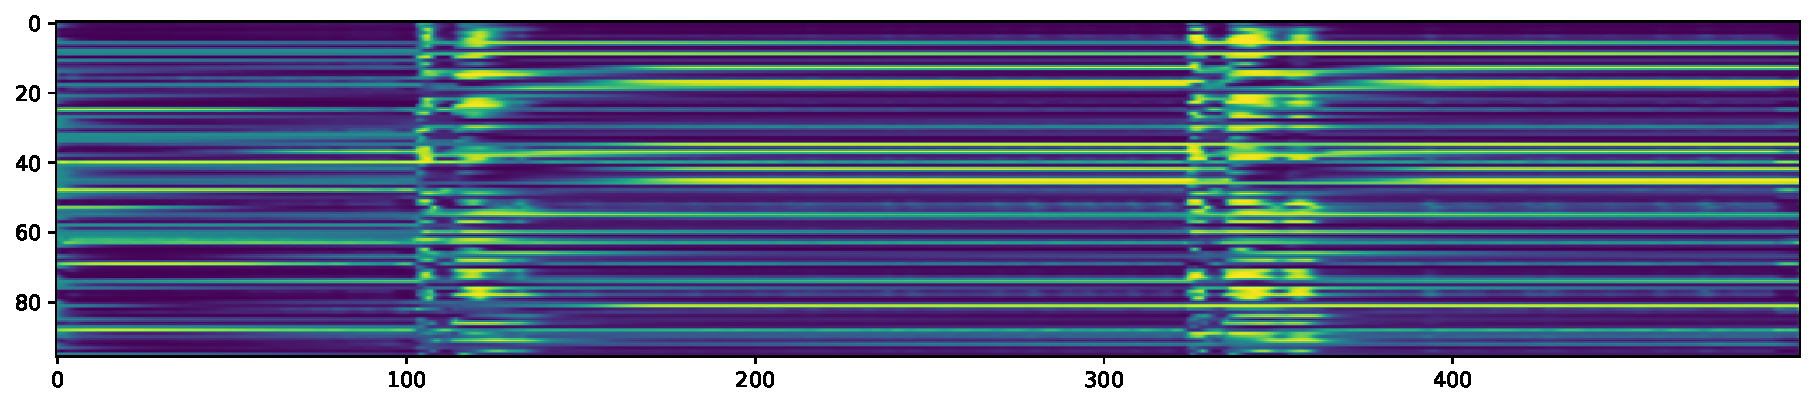
\includegraphics[width=\textwidth]{../images/crnn.gru.output.before.pooling.pdf}
            \caption{Image de sortie après la couche récurrente (GRU) avant la couche de pooling}
            \label{fig:crnn.gru.output.before.pooling}
        \end{subfigure}
        \hfill
        \begin{subfigure}[b]{0.45\textwidth}
            \centering
            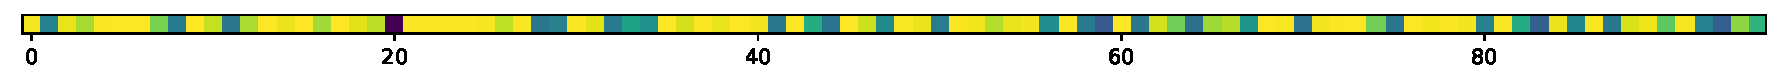
\includegraphics[width=\textwidth]{../images/crnn.gru.pooling.output.pdf}
            \caption{Image de sortie après la couche de pooling}
            \label{fig:crnn.gru.pooling.output}
        \end{subfigure}

        \vspace{0.5cm}

        \begin{subfigure}[b]{0.45\textwidth}
            \centering
            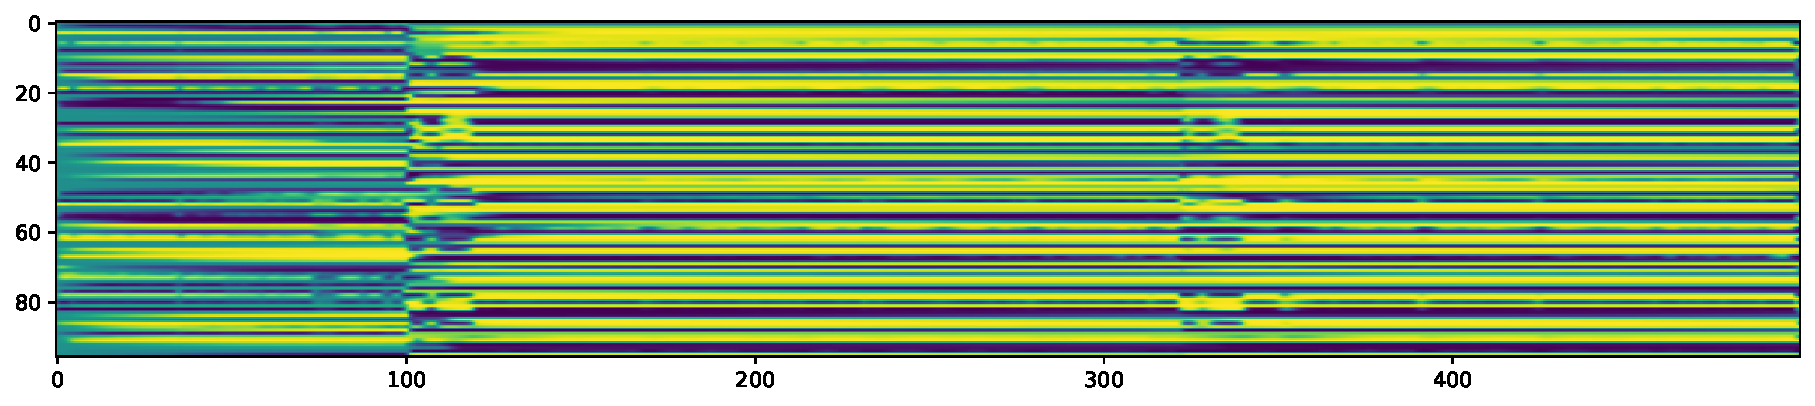
\includegraphics[width=\textwidth]{../images/crnn.gru.output.before.attention.pdf}
            \caption{Image de sortie après la couche récurrente (GRU) avant la couche d'attention}
            \label{fig:crnn.gru.output.before.attention}
        \end{subfigure}
        \hfill
        \begin{subfigure}[b]{0.45\textwidth}
            \centering
            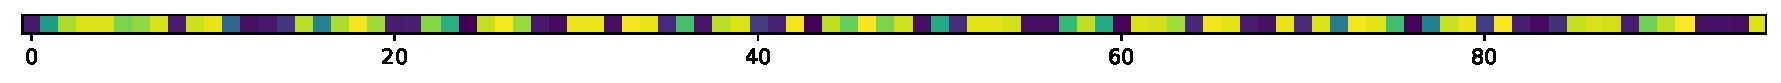
\includegraphics[width=\textwidth]{../images/crnn.gru.attention.output.pdf}
            \caption{Image de sortie après la couche d'attention}
            \label{fig:crnn.gru.attention.output}
        \end{subfigure}
    \end{figure}

    $\Rightarrow$ Ici, 99.9~\% de chances qu'un son d'oiseau soit présent dans l'audio.

\end{frame}

\section{Conclusion} \subsection{}

\begin{frame}{}

    \begin{block}{Qu'en tirer ?}
        \begin{itemize}
            \item Très exploratoire, chronophage, besoin de \textbf{faire des choix} dans ce que l'on veut faire.
            \item Envie d'approfondir les modèles attentionnels.
            \item Envie de \textbf{comprendre la théorie} derrière le traitement du signal.
        \end{itemize}
    \end{block}

    Merci !

\end{frame}

\section{Bibliographie} \subsection{}

\begin{frame}[allowframebreaks]{Bibliographie}

    \printbibliography[heading=none]

\end{frame}




\end{document}

